% Copyright © 2013 Martin Ueding <dev@martin-ueding.de>

% Copyright © 2012-2013 Martin Ueding <dev@martin-ueding.de>

% This is my general purpose LaTeX header file for writing German documents.
% Ideally, you include this using a simple ``% Copyright © 2012-2013 Martin Ueding <dev@martin-ueding.de>

% This is my general purpose LaTeX header file for writing German documents.
% Ideally, you include this using a simple ``% Copyright © 2012-2013 Martin Ueding <dev@martin-ueding.de>

% This is my general purpose LaTeX header file for writing German documents.
% Ideally, you include this using a simple ``\input{header.tex}`` in your main
% document and start with ``\title`` and ``\begin{document}`` afterwards.

% If you need to add additional packages, I recommend not doing this in this
% file, but in your main document. That way, you can just drop in a new
% ``header.tex`` and get all the new commands without having to merge manually.

% Since this file encorporates a CC-BY-SA fragment, this whole files is
% licensed under the CC-BY-SA license.

\documentclass[11pt, ngerman, fleqn, DIV=15, BCOR=2cm, headinclude]{scrartcl}

\usepackage{graphicx}

% Environment to quote the problem. Currently, this is just a new name for the
% quote environment.
\newenvironment{problem}{\begin{quote}\textsf{\textbf{Aufgabenstellung:}}\quad}{\end{quote}}

\setkomafont{caption}{\sf}
\setkomafont{captionlabel}{\usekomafont{caption}}

%%%%%%%%%%%%%%%%%%%%%%%%%%%%%%%%%%%%%%%%%%%%%%%%%%%%%%%%%%%%%%%%%%%%%%%%%%%%%%%
%                                Locale, date                                 %
%%%%%%%%%%%%%%%%%%%%%%%%%%%%%%%%%%%%%%%%%%%%%%%%%%%%%%%%%%%%%%%%%%%%%%%%%%%%%%%

\usepackage{babel}
\usepackage[iso]{isodate}

%%%%%%%%%%%%%%%%%%%%%%%%%%%%%%%%%%%%%%%%%%%%%%%%%%%%%%%%%%%%%%%%%%%%%%%%%%%%%%%
%                          Margins and other spacing                          %
%%%%%%%%%%%%%%%%%%%%%%%%%%%%%%%%%%%%%%%%%%%%%%%%%%%%%%%%%%%%%%%%%%%%%%%%%%%%%%%

\usepackage[parfill]{parskip}
\usepackage{setspace}
\usepackage[activate]{microtype}

\setlength{\columnsep}{2cm}

%%%%%%%%%%%%%%%%%%%%%%%%%%%%%%%%%%%%%%%%%%%%%%%%%%%%%%%%%%%%%%%%%%%%%%%%%%%%%%%
%                                    Color                                    %
%%%%%%%%%%%%%%%%%%%%%%%%%%%%%%%%%%%%%%%%%%%%%%%%%%%%%%%%%%%%%%%%%%%%%%%%%%%%%%%

\usepackage[usenames, dvipsnames]{xcolor}

\colorlet{darkred}{red!70!black}
\colorlet{darkblue}{blue!70!black}
\colorlet{darkgreen}{green!40!black}

%%%%%%%%%%%%%%%%%%%%%%%%%%%%%%%%%%%%%%%%%%%%%%%%%%%%%%%%%%%%%%%%%%%%%%%%%%%%%%%
%                         Font and font like settings                         %
%%%%%%%%%%%%%%%%%%%%%%%%%%%%%%%%%%%%%%%%%%%%%%%%%%%%%%%%%%%%%%%%%%%%%%%%%%%%%%%

% This replaces all fonts with Bitstream Charter, Bitstream Vera Sans and
% Bitstream Vera Mono. Math will be rendered in Charter.
\usepackage[charter, greekuppercase=italicized]{mathdesign}
\usepackage{beramono}
\usepackage{berasans}

% Bold, sans-serif tensors. This fragment is taken from “egreg” from
% http://tex.stackexchange.com/a/82747/8945 and licensed under `CC-BY-SA
% <https://creativecommons.org/licenses/by-sa/3.0/>`_.
\usepackage{bm}
\DeclareMathAlphabet{\mathsfit}{\encodingdefault}{\sfdefault}{m}{sl}
\SetMathAlphabet{\mathsfit}{bold}{\encodingdefault}{\sfdefault}{bx}{sl}
\newcommand{\tens}[1]{\bm{\mathsfit{#1}}}

% Bold vectors.
\renewcommand{\vec}[1]{\boldsymbol{#1}}

%%%%%%%%%%%%%%%%%%%%%%%%%%%%%%%%%%%%%%%%%%%%%%%%%%%%%%%%%%%%%%%%%%%%%%%%%%%%%%%
%                               Input encoding                                %
%%%%%%%%%%%%%%%%%%%%%%%%%%%%%%%%%%%%%%%%%%%%%%%%%%%%%%%%%%%%%%%%%%%%%%%%%%%%%%%

\usepackage[T1]{fontenc}
\usepackage[utf8]{inputenc}

%%%%%%%%%%%%%%%%%%%%%%%%%%%%%%%%%%%%%%%%%%%%%%%%%%%%%%%%%%%%%%%%%%%%%%%%%%%%%%%
%                         Hyperrefs and PDF metadata                          %
%%%%%%%%%%%%%%%%%%%%%%%%%%%%%%%%%%%%%%%%%%%%%%%%%%%%%%%%%%%%%%%%%%%%%%%%%%%%%%%

\usepackage{hyperref}
\usepackage{lastpage}

% This sets the author in the properties of the PDF as well. If you want to
% change it, just override it with another ``\hypersetup`` call.
\hypersetup{
	breaklinks=false,
	citecolor=darkgreen,
	colorlinks=true,
	linkcolor=darkblue,
	menucolor=black,
	pdfauthor={Martin Ueding},
	urlcolor=darkblue,
}

%%%%%%%%%%%%%%%%%%%%%%%%%%%%%%%%%%%%%%%%%%%%%%%%%%%%%%%%%%%%%%%%%%%%%%%%%%%%%%%
%                               Math Operators                                %
%%%%%%%%%%%%%%%%%%%%%%%%%%%%%%%%%%%%%%%%%%%%%%%%%%%%%%%%%%%%%%%%%%%%%%%%%%%%%%%

% AMS environments like ``align`` and theorems like ``proof``.
\usepackage{amsmath}
\usepackage{amsthm}

% Common math constructs like partial derivatives.
\usepackage{commath}

% Physical units.
\usepackage[output-decimal-marker={,}]{siunitx}

% Since I use mathdesign with italic uppercase greek characters, the Ohm unit will be displayed with an italic Ω by default. Units have to be roman, so this forces it the right way.
\DeclareSIUnit{\ohm}{$\Omegaup$}
\DeclareSIUnit{\division}{DIV}
\DeclareSIUnit{\voltss}{$\mathrm{V_{SS}}$}

% Word like operators.
\DeclareMathOperator{\acosh}{arcosh}
\DeclareMathOperator{\arcosh}{arcosh}
\DeclareMathOperator{\arcsinh}{arsinh}
\DeclareMathOperator{\arsinh}{arsinh}
\DeclareMathOperator{\asinh}{arsinh}
\DeclareMathOperator{\card}{card}
\DeclareMathOperator{\csch}{cshs}
\DeclareMathOperator{\diam}{diam}
\DeclareMathOperator{\sech}{sech}
\renewcommand{\Im}{\mathop{{}\mathrm{Im}}\nolimits}
\renewcommand{\Re}{\mathop{{}\mathrm{Re}}\nolimits}

% Fourier transform.
\DeclareMathOperator{\fourier}{\ensuremath{\mathcal{F}}}

% Roman versions of “e” and “i” to serve as Euler's number and the imaginary
% constant.
\newcommand{\ee}{\eup}
\newcommand{\eup}{\mathrm e}
\newcommand{\ii}{\iup}
\newcommand{\iup}{\mathrm i}

% Symbols for the various mathematical fields (natural numbers, integers,
% rational numbers, real numbers, complex numbers).
\newcommand{\C}{\ensuremath{\mathbb C}}
\newcommand{\N}{\ensuremath{\mathbb N}}
\newcommand{\Q}{\ensuremath{\mathbb Q}}
\newcommand{\R}{\ensuremath{\mathbb R}}
\newcommand{\Z}{\ensuremath{\mathbb Z}}

% Shape like operators.
\DeclareMathOperator{\dalambert}{\Box}
\DeclareMathOperator{\laplace}{\bigtriangleup}
\newcommand{\curl}{\vnabla \times}
\newcommand{\divergence}[1]{\inner{\vnabla}{#1}}
\newcommand{\vnabla}{\vec \nabla}

\newcommand{\half}{\frac 12}

% Unit vector (German „Einheitsvektor“).
\newcommand{\ev}{\hat{\vec e}}

% Scientific notation for large numbers.
\newcommand{\e}[1]{\cdot 10^{#1}}

% Mathematician's notation for the inner (scalar, dot) product.
\newcommand{\bracket}[1]{\left\langle #1 \right\rangle}
\newcommand{\inner}[2]{\bracket{#1, #2}}

% Placeholders.
\newcommand{\emesswert}{\del{\messwert \pm \messwert}}
\newcommand{\fehlt}{\textcolor{darkred}{Hier fehlen noch Inhalte.}}
\newcommand{\messwert}{\textcolor{blue}{\square}}
\newcommand{\punkte}{\phantom{xxxxx}}
\newcommand{\punktevon}[1]{\begin{flushright}/ #1\end{flushright}}

% Separator for equations on a single line.
\newcommand{\eqnsep}{,\quad}

% Quantum Mechanics
\usepackage{braket}

%%%%%%%%%%%%%%%%%%%%%%%%%%%%%%%%%%%%%%%%%%%%%%%%%%%%%%%%%%%%%%%%%%%%%%%%%%%%%%%
%                                  Headings                                   %
%%%%%%%%%%%%%%%%%%%%%%%%%%%%%%%%%%%%%%%%%%%%%%%%%%%%%%%%%%%%%%%%%%%%%%%%%%%%%%%

% This will set fancy headings to the top of the page. The page number will be
% accompanied by the total number of pages. That way, you will know if any page
% is missing.
%
% If you do not want this for your document, you can just use
% ``\pagestyle{plain}``.

\usepackage{scrpage2}

\pagestyle{scrheadings}
\automark{section}
\cfoot{\footnotesize{Seite \thepage\ / \pageref{LastPage}}}
\chead{}
\ihead{}
\ohead{\rightmark}
\setheadsepline{.4pt}

%%%%%%%%%%%%%%%%%%%%%%%%%%%%%%%%%%%%%%%%%%%%%%%%%%%%%%%%%%%%%%%%%%%%%%%%%%%%%%%
%                            Bibliography (BibTeX)                            %
%%%%%%%%%%%%%%%%%%%%%%%%%%%%%%%%%%%%%%%%%%%%%%%%%%%%%%%%%%%%%%%%%%%%%%%%%%%%%%%

\newcommand{\bibliographyfile}{../../central-bibtex/Central}
\bibliographystyle{apalike2}

%%%%%%%%%%%%%%%%%%%%%%%%%%%%%%%%%%%%%%%%%%%%%%%%%%%%%%%%%%%%%%%%%%%%%%%%%%%%%%%
%                                Abbreviations                                %
%%%%%%%%%%%%%%%%%%%%%%%%%%%%%%%%%%%%%%%%%%%%%%%%%%%%%%%%%%%%%%%%%%%%%%%%%%%%%%%

\newcommand{\dhabk}{\mbox{d.\,h.}}

%%%%%%%%%%%%%%%%%%%%%%%%%%%%%%%%%%%%%%%%%%%%%%%%%%%%%%%%%%%%%%%%%%%%%%%%%%%%%%%
%                                  Licences                                   %
%%%%%%%%%%%%%%%%%%%%%%%%%%%%%%%%%%%%%%%%%%%%%%%%%%%%%%%%%%%%%%%%%%%%%%%%%%%%%%%

\usepackage{ccicons}

\newcommand{\ccbysadetext}{%
	\begin{small}
		Dieses Werk bzw. Inhalt steht unter einer
		\href{http://creativecommons.org/licenses/by-sa/3.0/deed.de}{%
			Creative Commons Namensnennung - Weitergabe unter gleichen
		Bedingungen 3.0 Unported Lizenz}.
	\end{small}
}

\newcommand{\ccbysadetitle}{%
	Lizenz: \href{http://creativecommons.org/licenses/by-sa/3.0/deed.de}
	{CC-BY-SA 3.0 \ccbysa}
}
`` in your main
% document and start with ``\title`` and ``\begin{document}`` afterwards.

% If you need to add additional packages, I recommend not doing this in this
% file, but in your main document. That way, you can just drop in a new
% ``header.tex`` and get all the new commands without having to merge manually.

% Since this file encorporates a CC-BY-SA fragment, this whole files is
% licensed under the CC-BY-SA license.

\documentclass[11pt, ngerman, fleqn, DIV=15, BCOR=2cm, headinclude]{scrartcl}

\usepackage{graphicx}

% Environment to quote the problem. Currently, this is just a new name for the
% quote environment.
\newenvironment{problem}{\begin{quote}\textsf{\textbf{Aufgabenstellung:}}\quad}{\end{quote}}

\setkomafont{caption}{\sf}
\setkomafont{captionlabel}{\usekomafont{caption}}

%%%%%%%%%%%%%%%%%%%%%%%%%%%%%%%%%%%%%%%%%%%%%%%%%%%%%%%%%%%%%%%%%%%%%%%%%%%%%%%
%                                Locale, date                                 %
%%%%%%%%%%%%%%%%%%%%%%%%%%%%%%%%%%%%%%%%%%%%%%%%%%%%%%%%%%%%%%%%%%%%%%%%%%%%%%%

\usepackage{babel}
\usepackage[iso]{isodate}

%%%%%%%%%%%%%%%%%%%%%%%%%%%%%%%%%%%%%%%%%%%%%%%%%%%%%%%%%%%%%%%%%%%%%%%%%%%%%%%
%                          Margins and other spacing                          %
%%%%%%%%%%%%%%%%%%%%%%%%%%%%%%%%%%%%%%%%%%%%%%%%%%%%%%%%%%%%%%%%%%%%%%%%%%%%%%%

\usepackage[parfill]{parskip}
\usepackage{setspace}
\usepackage[activate]{microtype}

\setlength{\columnsep}{2cm}

%%%%%%%%%%%%%%%%%%%%%%%%%%%%%%%%%%%%%%%%%%%%%%%%%%%%%%%%%%%%%%%%%%%%%%%%%%%%%%%
%                                    Color                                    %
%%%%%%%%%%%%%%%%%%%%%%%%%%%%%%%%%%%%%%%%%%%%%%%%%%%%%%%%%%%%%%%%%%%%%%%%%%%%%%%

\usepackage[usenames, dvipsnames]{xcolor}

\colorlet{darkred}{red!70!black}
\colorlet{darkblue}{blue!70!black}
\colorlet{darkgreen}{green!40!black}

%%%%%%%%%%%%%%%%%%%%%%%%%%%%%%%%%%%%%%%%%%%%%%%%%%%%%%%%%%%%%%%%%%%%%%%%%%%%%%%
%                         Font and font like settings                         %
%%%%%%%%%%%%%%%%%%%%%%%%%%%%%%%%%%%%%%%%%%%%%%%%%%%%%%%%%%%%%%%%%%%%%%%%%%%%%%%

% This replaces all fonts with Bitstream Charter, Bitstream Vera Sans and
% Bitstream Vera Mono. Math will be rendered in Charter.
\usepackage[charter, greekuppercase=italicized]{mathdesign}
\usepackage{beramono}
\usepackage{berasans}

% Bold, sans-serif tensors. This fragment is taken from “egreg” from
% http://tex.stackexchange.com/a/82747/8945 and licensed under `CC-BY-SA
% <https://creativecommons.org/licenses/by-sa/3.0/>`_.
\usepackage{bm}
\DeclareMathAlphabet{\mathsfit}{\encodingdefault}{\sfdefault}{m}{sl}
\SetMathAlphabet{\mathsfit}{bold}{\encodingdefault}{\sfdefault}{bx}{sl}
\newcommand{\tens}[1]{\bm{\mathsfit{#1}}}

% Bold vectors.
\renewcommand{\vec}[1]{\boldsymbol{#1}}

%%%%%%%%%%%%%%%%%%%%%%%%%%%%%%%%%%%%%%%%%%%%%%%%%%%%%%%%%%%%%%%%%%%%%%%%%%%%%%%
%                               Input encoding                                %
%%%%%%%%%%%%%%%%%%%%%%%%%%%%%%%%%%%%%%%%%%%%%%%%%%%%%%%%%%%%%%%%%%%%%%%%%%%%%%%

\usepackage[T1]{fontenc}
\usepackage[utf8]{inputenc}

%%%%%%%%%%%%%%%%%%%%%%%%%%%%%%%%%%%%%%%%%%%%%%%%%%%%%%%%%%%%%%%%%%%%%%%%%%%%%%%
%                         Hyperrefs and PDF metadata                          %
%%%%%%%%%%%%%%%%%%%%%%%%%%%%%%%%%%%%%%%%%%%%%%%%%%%%%%%%%%%%%%%%%%%%%%%%%%%%%%%

\usepackage{hyperref}
\usepackage{lastpage}

% This sets the author in the properties of the PDF as well. If you want to
% change it, just override it with another ``\hypersetup`` call.
\hypersetup{
	breaklinks=false,
	citecolor=darkgreen,
	colorlinks=true,
	linkcolor=darkblue,
	menucolor=black,
	pdfauthor={Martin Ueding},
	urlcolor=darkblue,
}

%%%%%%%%%%%%%%%%%%%%%%%%%%%%%%%%%%%%%%%%%%%%%%%%%%%%%%%%%%%%%%%%%%%%%%%%%%%%%%%
%                               Math Operators                                %
%%%%%%%%%%%%%%%%%%%%%%%%%%%%%%%%%%%%%%%%%%%%%%%%%%%%%%%%%%%%%%%%%%%%%%%%%%%%%%%

% AMS environments like ``align`` and theorems like ``proof``.
\usepackage{amsmath}
\usepackage{amsthm}

% Common math constructs like partial derivatives.
\usepackage{commath}

% Physical units.
\usepackage[output-decimal-marker={,}]{siunitx}

% Since I use mathdesign with italic uppercase greek characters, the Ohm unit will be displayed with an italic Ω by default. Units have to be roman, so this forces it the right way.
\DeclareSIUnit{\ohm}{$\Omegaup$}
\DeclareSIUnit{\division}{DIV}
\DeclareSIUnit{\voltss}{$\mathrm{V_{SS}}$}

% Word like operators.
\DeclareMathOperator{\acosh}{arcosh}
\DeclareMathOperator{\arcosh}{arcosh}
\DeclareMathOperator{\arcsinh}{arsinh}
\DeclareMathOperator{\arsinh}{arsinh}
\DeclareMathOperator{\asinh}{arsinh}
\DeclareMathOperator{\card}{card}
\DeclareMathOperator{\csch}{cshs}
\DeclareMathOperator{\diam}{diam}
\DeclareMathOperator{\sech}{sech}
\renewcommand{\Im}{\mathop{{}\mathrm{Im}}\nolimits}
\renewcommand{\Re}{\mathop{{}\mathrm{Re}}\nolimits}

% Fourier transform.
\DeclareMathOperator{\fourier}{\ensuremath{\mathcal{F}}}

% Roman versions of “e” and “i” to serve as Euler's number and the imaginary
% constant.
\newcommand{\ee}{\eup}
\newcommand{\eup}{\mathrm e}
\newcommand{\ii}{\iup}
\newcommand{\iup}{\mathrm i}

% Symbols for the various mathematical fields (natural numbers, integers,
% rational numbers, real numbers, complex numbers).
\newcommand{\C}{\ensuremath{\mathbb C}}
\newcommand{\N}{\ensuremath{\mathbb N}}
\newcommand{\Q}{\ensuremath{\mathbb Q}}
\newcommand{\R}{\ensuremath{\mathbb R}}
\newcommand{\Z}{\ensuremath{\mathbb Z}}

% Shape like operators.
\DeclareMathOperator{\dalambert}{\Box}
\DeclareMathOperator{\laplace}{\bigtriangleup}
\newcommand{\curl}{\vnabla \times}
\newcommand{\divergence}[1]{\inner{\vnabla}{#1}}
\newcommand{\vnabla}{\vec \nabla}

\newcommand{\half}{\frac 12}

% Unit vector (German „Einheitsvektor“).
\newcommand{\ev}{\hat{\vec e}}

% Scientific notation for large numbers.
\newcommand{\e}[1]{\cdot 10^{#1}}

% Mathematician's notation for the inner (scalar, dot) product.
\newcommand{\bracket}[1]{\left\langle #1 \right\rangle}
\newcommand{\inner}[2]{\bracket{#1, #2}}

% Placeholders.
\newcommand{\emesswert}{\del{\messwert \pm \messwert}}
\newcommand{\fehlt}{\textcolor{darkred}{Hier fehlen noch Inhalte.}}
\newcommand{\messwert}{\textcolor{blue}{\square}}
\newcommand{\punkte}{\phantom{xxxxx}}
\newcommand{\punktevon}[1]{\begin{flushright}/ #1\end{flushright}}

% Separator for equations on a single line.
\newcommand{\eqnsep}{,\quad}

% Quantum Mechanics
\usepackage{braket}

%%%%%%%%%%%%%%%%%%%%%%%%%%%%%%%%%%%%%%%%%%%%%%%%%%%%%%%%%%%%%%%%%%%%%%%%%%%%%%%
%                                  Headings                                   %
%%%%%%%%%%%%%%%%%%%%%%%%%%%%%%%%%%%%%%%%%%%%%%%%%%%%%%%%%%%%%%%%%%%%%%%%%%%%%%%

% This will set fancy headings to the top of the page. The page number will be
% accompanied by the total number of pages. That way, you will know if any page
% is missing.
%
% If you do not want this for your document, you can just use
% ``\pagestyle{plain}``.

\usepackage{scrpage2}

\pagestyle{scrheadings}
\automark{section}
\cfoot{\footnotesize{Seite \thepage\ / \pageref{LastPage}}}
\chead{}
\ihead{}
\ohead{\rightmark}
\setheadsepline{.4pt}

%%%%%%%%%%%%%%%%%%%%%%%%%%%%%%%%%%%%%%%%%%%%%%%%%%%%%%%%%%%%%%%%%%%%%%%%%%%%%%%
%                            Bibliography (BibTeX)                            %
%%%%%%%%%%%%%%%%%%%%%%%%%%%%%%%%%%%%%%%%%%%%%%%%%%%%%%%%%%%%%%%%%%%%%%%%%%%%%%%

\newcommand{\bibliographyfile}{../../central-bibtex/Central}
\bibliographystyle{apalike2}

%%%%%%%%%%%%%%%%%%%%%%%%%%%%%%%%%%%%%%%%%%%%%%%%%%%%%%%%%%%%%%%%%%%%%%%%%%%%%%%
%                                Abbreviations                                %
%%%%%%%%%%%%%%%%%%%%%%%%%%%%%%%%%%%%%%%%%%%%%%%%%%%%%%%%%%%%%%%%%%%%%%%%%%%%%%%

\newcommand{\dhabk}{\mbox{d.\,h.}}

%%%%%%%%%%%%%%%%%%%%%%%%%%%%%%%%%%%%%%%%%%%%%%%%%%%%%%%%%%%%%%%%%%%%%%%%%%%%%%%
%                                  Licences                                   %
%%%%%%%%%%%%%%%%%%%%%%%%%%%%%%%%%%%%%%%%%%%%%%%%%%%%%%%%%%%%%%%%%%%%%%%%%%%%%%%

\usepackage{ccicons}

\newcommand{\ccbysadetext}{%
	\begin{small}
		Dieses Werk bzw. Inhalt steht unter einer
		\href{http://creativecommons.org/licenses/by-sa/3.0/deed.de}{%
			Creative Commons Namensnennung - Weitergabe unter gleichen
		Bedingungen 3.0 Unported Lizenz}.
	\end{small}
}

\newcommand{\ccbysadetitle}{%
	Lizenz: \href{http://creativecommons.org/licenses/by-sa/3.0/deed.de}
	{CC-BY-SA 3.0 \ccbysa}
}
`` in your main
% document and start with ``\title`` and ``\begin{document}`` afterwards.

% If you need to add additional packages, I recommend not doing this in this
% file, but in your main document. That way, you can just drop in a new
% ``header.tex`` and get all the new commands without having to merge manually.

% Since this file encorporates a CC-BY-SA fragment, this whole files is
% licensed under the CC-BY-SA license.

\documentclass[11pt, ngerman, fleqn, DIV=15, BCOR=2cm, headinclude]{scrartcl}

\usepackage{graphicx}

% Environment to quote the problem. Currently, this is just a new name for the
% quote environment.
\newenvironment{problem}{\begin{quote}\textsf{\textbf{Aufgabenstellung:}}\quad}{\end{quote}}

\setkomafont{caption}{\sf}
\setkomafont{captionlabel}{\usekomafont{caption}}

%%%%%%%%%%%%%%%%%%%%%%%%%%%%%%%%%%%%%%%%%%%%%%%%%%%%%%%%%%%%%%%%%%%%%%%%%%%%%%%
%                                Locale, date                                 %
%%%%%%%%%%%%%%%%%%%%%%%%%%%%%%%%%%%%%%%%%%%%%%%%%%%%%%%%%%%%%%%%%%%%%%%%%%%%%%%

\usepackage{babel}
\usepackage[iso]{isodate}

%%%%%%%%%%%%%%%%%%%%%%%%%%%%%%%%%%%%%%%%%%%%%%%%%%%%%%%%%%%%%%%%%%%%%%%%%%%%%%%
%                          Margins and other spacing                          %
%%%%%%%%%%%%%%%%%%%%%%%%%%%%%%%%%%%%%%%%%%%%%%%%%%%%%%%%%%%%%%%%%%%%%%%%%%%%%%%

\usepackage[parfill]{parskip}
\usepackage{setspace}
\usepackage[activate]{microtype}

\setlength{\columnsep}{2cm}

%%%%%%%%%%%%%%%%%%%%%%%%%%%%%%%%%%%%%%%%%%%%%%%%%%%%%%%%%%%%%%%%%%%%%%%%%%%%%%%
%                                    Color                                    %
%%%%%%%%%%%%%%%%%%%%%%%%%%%%%%%%%%%%%%%%%%%%%%%%%%%%%%%%%%%%%%%%%%%%%%%%%%%%%%%

\usepackage[usenames, dvipsnames]{xcolor}

\colorlet{darkred}{red!70!black}
\colorlet{darkblue}{blue!70!black}
\colorlet{darkgreen}{green!40!black}

%%%%%%%%%%%%%%%%%%%%%%%%%%%%%%%%%%%%%%%%%%%%%%%%%%%%%%%%%%%%%%%%%%%%%%%%%%%%%%%
%                         Font and font like settings                         %
%%%%%%%%%%%%%%%%%%%%%%%%%%%%%%%%%%%%%%%%%%%%%%%%%%%%%%%%%%%%%%%%%%%%%%%%%%%%%%%

% This replaces all fonts with Bitstream Charter, Bitstream Vera Sans and
% Bitstream Vera Mono. Math will be rendered in Charter.
\usepackage[charter, greekuppercase=italicized]{mathdesign}
\usepackage{beramono}
\usepackage{berasans}

% Bold, sans-serif tensors. This fragment is taken from “egreg” from
% http://tex.stackexchange.com/a/82747/8945 and licensed under `CC-BY-SA
% <https://creativecommons.org/licenses/by-sa/3.0/>`_.
\usepackage{bm}
\DeclareMathAlphabet{\mathsfit}{\encodingdefault}{\sfdefault}{m}{sl}
\SetMathAlphabet{\mathsfit}{bold}{\encodingdefault}{\sfdefault}{bx}{sl}
\newcommand{\tens}[1]{\bm{\mathsfit{#1}}}

% Bold vectors.
\renewcommand{\vec}[1]{\boldsymbol{#1}}

%%%%%%%%%%%%%%%%%%%%%%%%%%%%%%%%%%%%%%%%%%%%%%%%%%%%%%%%%%%%%%%%%%%%%%%%%%%%%%%
%                               Input encoding                                %
%%%%%%%%%%%%%%%%%%%%%%%%%%%%%%%%%%%%%%%%%%%%%%%%%%%%%%%%%%%%%%%%%%%%%%%%%%%%%%%

\usepackage[T1]{fontenc}
\usepackage[utf8]{inputenc}

%%%%%%%%%%%%%%%%%%%%%%%%%%%%%%%%%%%%%%%%%%%%%%%%%%%%%%%%%%%%%%%%%%%%%%%%%%%%%%%
%                         Hyperrefs and PDF metadata                          %
%%%%%%%%%%%%%%%%%%%%%%%%%%%%%%%%%%%%%%%%%%%%%%%%%%%%%%%%%%%%%%%%%%%%%%%%%%%%%%%

\usepackage{hyperref}
\usepackage{lastpage}

% This sets the author in the properties of the PDF as well. If you want to
% change it, just override it with another ``\hypersetup`` call.
\hypersetup{
	breaklinks=false,
	citecolor=darkgreen,
	colorlinks=true,
	linkcolor=darkblue,
	menucolor=black,
	pdfauthor={Martin Ueding},
	urlcolor=darkblue,
}

%%%%%%%%%%%%%%%%%%%%%%%%%%%%%%%%%%%%%%%%%%%%%%%%%%%%%%%%%%%%%%%%%%%%%%%%%%%%%%%
%                               Math Operators                                %
%%%%%%%%%%%%%%%%%%%%%%%%%%%%%%%%%%%%%%%%%%%%%%%%%%%%%%%%%%%%%%%%%%%%%%%%%%%%%%%

% AMS environments like ``align`` and theorems like ``proof``.
\usepackage{amsmath}
\usepackage{amsthm}

% Common math constructs like partial derivatives.
\usepackage{commath}

% Physical units.
\usepackage[output-decimal-marker={,}]{siunitx}

% Since I use mathdesign with italic uppercase greek characters, the Ohm unit will be displayed with an italic Ω by default. Units have to be roman, so this forces it the right way.
\DeclareSIUnit{\ohm}{$\Omegaup$}
\DeclareSIUnit{\division}{DIV}
\DeclareSIUnit{\voltss}{$\mathrm{V_{SS}}$}

% Word like operators.
\DeclareMathOperator{\acosh}{arcosh}
\DeclareMathOperator{\arcosh}{arcosh}
\DeclareMathOperator{\arcsinh}{arsinh}
\DeclareMathOperator{\arsinh}{arsinh}
\DeclareMathOperator{\asinh}{arsinh}
\DeclareMathOperator{\card}{card}
\DeclareMathOperator{\csch}{cshs}
\DeclareMathOperator{\diam}{diam}
\DeclareMathOperator{\sech}{sech}
\renewcommand{\Im}{\mathop{{}\mathrm{Im}}\nolimits}
\renewcommand{\Re}{\mathop{{}\mathrm{Re}}\nolimits}

% Fourier transform.
\DeclareMathOperator{\fourier}{\ensuremath{\mathcal{F}}}

% Roman versions of “e” and “i” to serve as Euler's number and the imaginary
% constant.
\newcommand{\ee}{\eup}
\newcommand{\eup}{\mathrm e}
\newcommand{\ii}{\iup}
\newcommand{\iup}{\mathrm i}

% Symbols for the various mathematical fields (natural numbers, integers,
% rational numbers, real numbers, complex numbers).
\newcommand{\C}{\ensuremath{\mathbb C}}
\newcommand{\N}{\ensuremath{\mathbb N}}
\newcommand{\Q}{\ensuremath{\mathbb Q}}
\newcommand{\R}{\ensuremath{\mathbb R}}
\newcommand{\Z}{\ensuremath{\mathbb Z}}

% Shape like operators.
\DeclareMathOperator{\dalambert}{\Box}
\DeclareMathOperator{\laplace}{\bigtriangleup}
\newcommand{\curl}{\vnabla \times}
\newcommand{\divergence}[1]{\inner{\vnabla}{#1}}
\newcommand{\vnabla}{\vec \nabla}

\newcommand{\half}{\frac 12}

% Unit vector (German „Einheitsvektor“).
\newcommand{\ev}{\hat{\vec e}}

% Scientific notation for large numbers.
\newcommand{\e}[1]{\cdot 10^{#1}}

% Mathematician's notation for the inner (scalar, dot) product.
\newcommand{\bracket}[1]{\left\langle #1 \right\rangle}
\newcommand{\inner}[2]{\bracket{#1, #2}}

% Placeholders.
\newcommand{\emesswert}{\del{\messwert \pm \messwert}}
\newcommand{\fehlt}{\textcolor{darkred}{Hier fehlen noch Inhalte.}}
\newcommand{\messwert}{\textcolor{blue}{\square}}
\newcommand{\punkte}{\phantom{xxxxx}}
\newcommand{\punktevon}[1]{\begin{flushright}/ #1\end{flushright}}

% Separator for equations on a single line.
\newcommand{\eqnsep}{,\quad}

% Quantum Mechanics
\usepackage{braket}

%%%%%%%%%%%%%%%%%%%%%%%%%%%%%%%%%%%%%%%%%%%%%%%%%%%%%%%%%%%%%%%%%%%%%%%%%%%%%%%
%                                  Headings                                   %
%%%%%%%%%%%%%%%%%%%%%%%%%%%%%%%%%%%%%%%%%%%%%%%%%%%%%%%%%%%%%%%%%%%%%%%%%%%%%%%

% This will set fancy headings to the top of the page. The page number will be
% accompanied by the total number of pages. That way, you will know if any page
% is missing.
%
% If you do not want this for your document, you can just use
% ``\pagestyle{plain}``.

\usepackage{scrpage2}

\pagestyle{scrheadings}
\automark{section}
\cfoot{\footnotesize{Seite \thepage\ / \pageref{LastPage}}}
\chead{}
\ihead{}
\ohead{\rightmark}
\setheadsepline{.4pt}

%%%%%%%%%%%%%%%%%%%%%%%%%%%%%%%%%%%%%%%%%%%%%%%%%%%%%%%%%%%%%%%%%%%%%%%%%%%%%%%
%                            Bibliography (BibTeX)                            %
%%%%%%%%%%%%%%%%%%%%%%%%%%%%%%%%%%%%%%%%%%%%%%%%%%%%%%%%%%%%%%%%%%%%%%%%%%%%%%%

\newcommand{\bibliographyfile}{../../central-bibtex/Central}
\bibliographystyle{apalike2}

%%%%%%%%%%%%%%%%%%%%%%%%%%%%%%%%%%%%%%%%%%%%%%%%%%%%%%%%%%%%%%%%%%%%%%%%%%%%%%%
%                                Abbreviations                                %
%%%%%%%%%%%%%%%%%%%%%%%%%%%%%%%%%%%%%%%%%%%%%%%%%%%%%%%%%%%%%%%%%%%%%%%%%%%%%%%

\newcommand{\dhabk}{\mbox{d.\,h.}}

%%%%%%%%%%%%%%%%%%%%%%%%%%%%%%%%%%%%%%%%%%%%%%%%%%%%%%%%%%%%%%%%%%%%%%%%%%%%%%%
%                                  Licences                                   %
%%%%%%%%%%%%%%%%%%%%%%%%%%%%%%%%%%%%%%%%%%%%%%%%%%%%%%%%%%%%%%%%%%%%%%%%%%%%%%%

\usepackage{ccicons}

\newcommand{\ccbysadetext}{%
	\begin{small}
		Dieses Werk bzw. Inhalt steht unter einer
		\href{http://creativecommons.org/licenses/by-sa/3.0/deed.de}{%
			Creative Commons Namensnennung - Weitergabe unter gleichen
		Bedingungen 3.0 Unported Lizenz}.
	\end{small}
}

\newcommand{\ccbysadetitle}{%
	Lizenz: \href{http://creativecommons.org/licenses/by-sa/3.0/deed.de}
	{CC-BY-SA 3.0 \ccbysa}
}


\usepackage{keystroke}
\usepackage{placeins}

\newcommand\versuchsnummer{402}

\ihead{physik412 – Versuch \versuchsnummer}
\ifoot{Martin Ueding, Lino Lemmer}

\subject{Praktikumsprotokoll}
\title{Quantelung von Energie}
\subtitle{physik412 – Versuch \versuchsnummer}
\author{
    Martin Ueding \\
    \small{\href{mailto:mu@martin-ueding.de}{mu@martin-ueding.de}}
    \and
    Lino Lemmer \\
    \small{\href{mailto:s6lilemm@uni-bonn.de}{s6lilemm@uni-bonn.de}}
}

%\setcounter{tocdepth}{2}

\newcommand\omegaG{\omega_\text G}
\newcommand\omegaB{\omega_\text B}

\begin{document}

\maketitle

\begin{abstract}
    In diesem Versuch wird im ersten Teil mit Hilfe des Photoeffektes das
    Placksche Wirkungsquantum abgeschätzt. Im zweiten Teil wird die
    Balmer-Serie von Wasserstoff und Deuterium untersucht und durch diese
    ebenfalls das Plancksche Wirkungsquantum bestimmt. Die so erhaltenen Werte
    für das Wirkungsquantum werden verglichen.
\end{abstract}

\tableofcontents

%%%%%%%%%%%%%%%%%%%%%%%%%%%%%%%%%%%%%%%%%%%%%%%%%%%%%%%%%%%%%%%%%%%%%%%%%%%%%%%
%                                   Theorie                                   %
%%%%%%%%%%%%%%%%%%%%%%%%%%%%%%%%%%%%%%%%%%%%%%%%%%%%%%%%%%%%%%%%%%%%%%%%%%%%%%%

\FloatBarrier
\section{Theorie}

Symbole:

\begin{itemize}

    \item Bankwinkel $\omega_\text B$
    \item Brennweite $f$
    \item Gitterkonstante $g$
    \item Gitterwinkel $\omega_\text G$
    \item Linienaufspaltung $d$
    \item Wellenlänge $\lambda$
    \item Wirkungsquantum $h$

\end{itemize}

\subsection{Photoeffekt}

Hinreichend kurzwelliges, also energiereiches Licht ist in der Lage, Elektronen
aus der Oberfläche eines Metalls auszulösen, indem einzelne Lichtquanten ihre
Energie $E = h\nu$ vollständig an ein Elektron im Metall abgeben. Die Energie
muss dabei die Austrittsarbeit $W_\text{A}$ Übersteigen, die übrige Energie
behält das Elektron in Form von kinetischer Energie. Die Menge der ausgelösten
Elektronen hängt dabei von der Intensität des Lichtes ab.

\subsection{Photozelle}

Der Aufbau einer Fotozelle ist in Abbildung~\ref{fig:Photozelle} zu sehen.

\begin{figure}
    \centering
    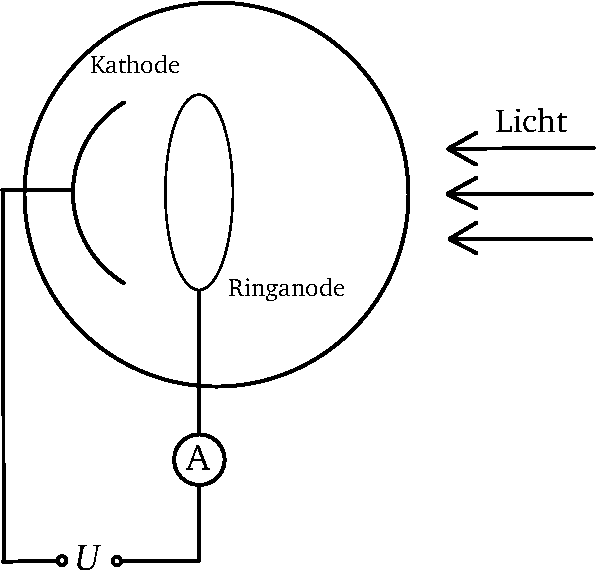
\includegraphics{../Zeichnungen/Photozelle.pdf}
    \caption{%
        Aufbau einer Photozelle mit Amperemeter und Gegenspannung $U$
    }
    \label{fig:Photozelle}
\end{figure}

In einem evakuiertem Behälter befinden sich eine Kathode und eine Ringanode,
zwischen denen eine Spannung anliegt. Die Anordnung wird mit Licht bestrahlt,
wodurch aus der Kathode Elektronen ausgelöst werden.

Liegt nun an der Kathode ein negatives und an der Anode ein positives Potenzial
an, werden die gelösten Elektronen in Richtung Anode beschleunigt. Mit dem
Amperemeter wird dann ein Strom gemessen.

Sind Kathode und Anode anders herum beschaltet, werden ausgelöste Elektronen in
Richtung Kathode beschleunigt, also abgebremst. Mit Hilfe der Spannung $U_0$,
bei der der Anodenstrom verschwindet, kann nun die kinetische Energie der
ausgelösten Elektronen bestimmt werden:

\[eU_0 = E_\text{kin}\]

Da die kinetische Energie die Differenz aus der Energie des Photons und der
Austrittsarbeit ist, gilt:

\[eU_0 = h\nu-W_\text{A}\]

Da man ein Auslösen von Elektronen aus der Anode verhindern möchte, wählt man
hier meist ein Material mit höherer Austrittsarbeit. Da so zwei Materialien mit
unterschiedlicher Austrittsarbeit verbunden sind, entsteht ein
Kontaktpotenzial, welches die Energiegleichung noch einmal verändert:

\begin{equation}
    U_0 = \frac he\nu - \frac{W_\text{A}}e - U_\text{K}
    \label{eq:Energiebilanz}
\end{equation}

Wenn man die Abhängigkeit der Gegenspannung $U_0$ von der Lichtfrequenz $\nu$
vermisst taucht das Konktaktpotenzial als Fehler bei der Bestimmung der
Austrittsarbeit (Achsenabschnitt) auf.

\subsection{Aufbau der Atomhülle}

\subsection{Spektroskopie}

\subsubsection{Gittergleichung}

Für die Bestimmung der Gitterkonstante im zweiten Versuchsteil wird eine
Gittergleichung benötigt, die nicht in der Anleitung gegeben ist. Diese muss
eine Gleichung sein, die die Abhängigkeit $(\omega_\text B, \omega_\text G,
\lambda) \mapsto g$ liefert.

Der Gangunterschied $\Delta$ bei einem Einfallswinkel $\alpha_0$ und einem
Austrittswinkel $\alpha_m$ für das Interferenzbild der Ordnung $m$ ist gegeben
durch: \cite[Formel~368.16]{physik312-Anleitung}
\begin{equation}
    \label{eq:368.16}
    \Delta = g \cdot \del{\sin(\alpha_0) + \sin(-\alpha_m)} = m \lambda
\end{equation}

In diesem Versuch haben wir ein Reflexionsgitter, außerdem sind die Messwerte
$\omega_\text B$ und $\omega_\text G$. Die Umrechnung ist wie folgt:
\[
    \alpha_0 = \omega_\text G
    \eqnsep
    \alpha_m = \piup - \del{ \omega_\text B + \omega_\text G }
\]

Dies setzen wir in \eqref{eq:368.16} ein und erhalten:
\begin{equation}
    \label{eq:gittergleichung}
    g = \frac{m \lambda}{\sin(\omega_\text G) - \sin(\omega_\text B + \omega_\text G)}
\end{equation}

Sollte $\omega_\text B = \piup$ sein, darf es keinen Gangunterschied geben.
$\Delta$ wird 0. Die Vorzeichen sind also korrekt.

\subsubsection{CCD-Kamera}

Die CCD-Kamera misst die Intensität für verschiedene Pixel. Aus den Pixeln
berechnet sie den Winkel bei der Objektivbrennweite $f$ und Pixelnummer $p \in
[0, 2047]$ mit folgender Formel:
\[
    \beta = \arctan\del{\frac{(1024 - p) \cdot \SI{0.014}{\milli\meter}}f}
\]

%%%%%%%%%%%%%%%%%%%%%%%%%%%%%%%%%%%%%%%%%%%%%%%%%%%%%%%%%%%%%%%%%%%%%%%%%%%%%%%
%                 Bestimmung des Planckschen Wirkungsquantums                 %
%%%%%%%%%%%%%%%%%%%%%%%%%%%%%%%%%%%%%%%%%%%%%%%%%%%%%%%%%%%%%%%%%%%%%%%%%%%%%%%

\FloatBarrier
\section{Bestimmung des Planckschen Wirkungsquantums}

\FloatBarrier
\subsection{Aufbau}

\begin{figure}[htbp]
    \centering
    %\includegraphics[width=\linewidth]{}
    \caption{%
        \cite[Abbildung~P402.1]{physik412-Anleitung}
    }
    \label{fig:P402.1}
\end{figure}

\FloatBarrier
\subsubsection{Justage}

Die Schutzkappe der Photozelle wird gelöst und das Filterrad auf $\lambda =
\SI{578}{\nano\meter}$ gestellt. Wenn die Hg-Dampflampe ihre volle Intensität
erreicht hat, können die Reflektionen auf Irisblende, Linse und
Interferenzfilter genutzt werden, um die Bauteile senkrecht und auf gleiche
Höhe auszurichten. Nun wird die Irisblende am Filterrad vollständig geöffnet
und die an der Lampe soweit geschlossen, dass der Lichtfleck auf der
Photokathode \SI{5}{\milli\meter} - \SI{10}{\milli\meter} Durchmesser hat.
Dabei soll die Ringanode nicht beleuchtet werden. Die Linse wird so verschoben,
dass der Lichfleck scharf abgebildet wird.

Im Anschluss wird die Schutzkappe so über die Photozelle gestülpt, dass
die Öffnung im Strahlengang liegt und die Irisblenden werden so weit
geschlossen, dass die Öffnung der Schutzkappe nicht überstrahlt wird.
Zuletzt wird, ohne dass die Justierung verändert wird, das Streulicht
begrenzende Rohr zwischen Schutzkappe und Filterrad angebracht.

\FloatBarrier
\subsubsection{Anschlüsse}

Der Anodenanschluss der Photozelle wird am negativen, der Kathodenanschluss am
positiven Ausgang eines Spannungsteilers angeschlossen, letzterer wird auf
Masse gezogen. Zwischen den Ausgängen wird ein Spannungsmesser angebracht. Der
Spannungsteiler liegt an einem regelbaren Netzgerät mit maximal \SI{12}{\volt}.

\FloatBarrier
\subsection{Durchführung}

Der Interferenzfilter wird auf das kurzwelligste Licht gestellt und die
Gegenspannung solange variiert, bis der Photostrom verschwindet. Nun wird der
Spannungsteiler so eingestellt, dass von da an die Maximalspannung etwa gleich
der gerade ermittelten Spannung ist. Für uns war das Verhältnis
$\frac{100}{550}$. Diese Einstellung wird für alle Messungen
beibehalten.

Nun wird zunächst der kleinste erreichbare Strom eingestellt. Dies ist $I_0$.
Die so eingestellte Gegenspannung ist ein erster Schätzwert für $U_0$.

Für die Kennlinie nimmt man Messpunkte von $U = \SI0{\volt}$ in
\SI{0.1}{\volt}-Abständen auf, bis $I = \SI0{\ampere}$ erreicht wird und geht
dann wieder mit gleichen Abständen zurück bis $U = \SI{0}{\volt}$.

Die Messungen für $I_0$, $U_0$ und die Kennlinie wird für alle Wellenlängen des
Filterrades durchgeführt.

Zuletzt wird mit veränderter Lichtintensität, bei deutlicher Vergrößerung bzw.
deutlicher Verringerung des Photostroms die Kennlinie der Wellenlänge $\lambda
= \SI{365}{\nano\meter}$ aufgenommem.

%TODO: Messdaten Teil 1 einfügen

\FloatBarrier
\subsection{Auswertung}

%%%%%%%%%%%%%%%%%%%%%%%%%%%%%%%%%%%%%%%%%%%%%%%%%%%%%%%%%%%%%%%%%%%%%%%%%%%%%%%
%                                Balmer-Serie                                 %
%%%%%%%%%%%%%%%%%%%%%%%%%%%%%%%%%%%%%%%%%%%%%%%%%%%%%%%%%%%%%%%%%%%%%%%%%%%%%%%

\FloatBarrier
\section{Balmer-Serie}

In diesem Versuchsteil untersuchen wir die Balmer-Serie einer
Wasserstoff-Deuterium-Lampe mit einem Reflexionsgitter.

\FloatBarrier
\subsection{Aufbau}

Auf einer optischen Bank mit zwei Armen, deren gegenseitige Lage mit einer
Winkelskala bestimmt werden kann, werden die Komponenten aufgebaut. Dabei wird
auf dem ersten Arm die Lampe, eine Linse mit $f = \SI{50}{\milli\meter}$, ein
einstellbarer Spalt sowie ein Objektiv mit $f = \SI{150}{\milli\meter}$
aufgebaut.

In die Mitte wird das holographische Reflexionsgitter angebracht.

Auf dem zweiten Arm wird von der Mitte aus eine Linse mit $f =
\SI{300}{\milli\meter}$ und ein Okular mit Strichskala angebracht. Im weiteren
Verlauf dieses Teilversuchs wird noch eine CCD-Kamera angebracht.

\FloatBarrier
\subsubsection{Justierung}

Zuerst müssen wir den Aufbau justieren. Dazu benutzen wir die helle
Quecksilberlampe. Diese wird an das Ende des einen Arms gesetzt. Mit der ersten
Linse bilden wir die Lampe auf den Spalt ab. Der Spalt ist so angebracht, dass
die schrägen Flanken zur Lichtquelle ausgerichtet sind, und dass der Spalt
senkrecht ist.

Wir setzen das Objektiv zwischen Spalt und Gitter ein und drehen das Gitter so,
dass die Reflexion des Gitters wieder durch das Objektiv fällt und auf den
Spalt trifft. Der Abstand von Objektiv und Spalt ist grob dessen Brennweite $f
= \SI{150}{\milli\meter}$. Mit Hilfe dieser Autokollimationsanordnung stellen
wir die Position des Objektivs so ein, dass das Bild des Spaltes scharf ist.
Dadurch ist der Strahlengang nach dem Objektiv auf unendlich fokussiert.

Nun ist das Bild scharf eingestellt, liegt aber noch ein wenig neben dem Spalt.
Daher drehen wir jetzt das Gitter mit den Rändelschrauben so, dass das Bild
exakt in den Spalt fällt.

Die optische Bank klappen wir nun so zu, dass der Winkel $\omega_\text B$ im
Bereich von \SIrange{130}{170}{\degree} liegt.

Das Okular wird ans Ende des anderen Armes gestellt und so justiert, dass einer
von uns die Skala gut ablesen kann. Zuletzt setzen wir die Linse mit $f =
\SI{300}{\milli\meter}$ ein, damit wir im zweiten Arm die Spektrallinien durch
ein Teleskop beobachten können.

\FloatBarrier
\subsection{Durchführung}

\FloatBarrier
\subsubsection{Bestimmung der Gitterkonstanten}
\label{sec:gitterkonstante/durchführung}

Wir bestimmen die Gitterkonstante des Gitters durch eine Messung mit einer
Quecksilberdampflampe. Dazu lösen wir die Rändelschraube der Gittersäule und
drehen so lange, bis die erste Linie sichtbar wird. Um die Linie einfacher
erkennen zu können, weiten wir den Spalt auf und stellen ihn anschließend auf
\SI{0.1}{\milli\meter} zurück.

Mit der Objektivlinse des Beobachtungsteleskops können wir die Linien
scharfstellen, wir justieren so lange, bis diese es sind. Dann lesen wir den
Winkel zwischen den Armen $\omega_\text B$ sowie den Winkel des Gitters
$\omega_\text G$ ab. Die gemessenen Winkel sind in
Tabelle~\ref{tab:messdaten:gitterkonstante}.

Im Anhang der Praktikumsanleitung ist das Spektrum der Quecksilberlampe
angegeben. Diese Tabelle zitieren wir im Anhang~\ref{sec:spektrum}.

\begin{table}[htbp]
    \centering
    \begin{tabular}{SSS}
        {Wellenlänge $\lambda / \si\meter$} & {Winkel $\omega_\text B /
    \si\radian$}  & {Winkel $\omega_\text G / \si\radian$} \\
        \hline
        % TODO Messdaten aus Datei laden.
    \end{tabular}
    \caption{%
        Messdaten für die Bestimmung der Gitterkonstanten mit der
        Quecksilberlampe.
    }
    \label{tab:messdaten:gitterkonstante}
\end{table}

\FloatBarrier
\subsubsection{Untersuchung der Balmer-Linien mit einem Okular}

Jetzt wiederholen wir diese Messung, jedoch mit der Balmer-Lampe. Dazu
entfernen wir die Quecksilberlampe und setzen die Wasserstofflampe ein. Mit der
ersten Linie bilden wir wieder die Lampe auf den Spalt ab. Dann führen die
gleiche Autokollimation wie im vorherigen Teil durch.

Die Rändelschraube an der Gittersäule wird gelöst und so weit gedreht, bis die
rote $\mathrm H_\alpha$-Linie zu sehen ist. Mit der Objektivlinse bilden wir
die Linie scharf ab.

Anschließend lesen wir die beiden Winkel ab. Außerdem schätzen wir den Abstand
$d$ der aufgespaltenen Linien mit Hilfe der Skala im Okular ab. Dann
wiederholen wir dies für alle anderen Linien. Unsere Messdaten sind in
Tabelle~\ref{tab:messdaten:balmer-okular}.

\begin{table}[htbp]
    \centering
    \begin{tabular}{SSSS}
        {Wellenlänge $\lambda / \si\meter$} & {Winkel $\omega_\text B / \si\radian$}  & {Winkel $\omega_\text G / \si\radian$} & {Aufspaltung $d / \si{\milli\meter}$} \\
        \hline
        % TODO Messdaten aus Datei laden.
    \end{tabular}
    \caption{%
        Messdaten für die Balmer-Lampe, bestimmt mit einem Okular
    }
    \label{tab:messdaten:balmer-okular}
\end{table}

\FloatBarrier
\subsubsection{Untersuchung der Balmer-Linien mit einer CCD-Kamera}

Jetzt wird das Okular durch eine CCD-Kamera ersetzt. Wir starten das Programm
„VideoCom“ und stellen im Menü „Kalibrierung / Theorievergleich“
(\keystroke{F5}) im Register „Beugungswinkel“ die Brennweite $f =
\SI{300}{\milli\meter}$ der Objektivlinse ein. Die Belichtungszeit stellen wir
auf Stufe 8. Wir aktivieren die Messung mit \keystroke{F9}.

Die roten Balmer-Linien müssen auf die Mitte der CCD-Zeile abgebildet werden,
daher drehen wir das Gitter entsprechend. Mit der Objektivlinse stellen wir die
Linien scharf, das Ergebnis kontrollieren wir auf dem Monitor.

Mit \Alt\keystroke{Z} vergrößern wir den Bereich und können die Aufspaltung so
besser erkennen.

Mit der Schaltfläche „$\sum_1$“ starten wir die Mittelwertsbildung. Sobald wir
mit dem Ergebnis zufrieden sind, stoppen wir die Messung mit \keystroke{F9}.
Die Messdatentabelle speichern wir mit „Tabelle Kopieren“ in einer Textdatei.
Zuletzt notieren wir die Winkel.

Diesen Vorgang wiederholen wir für alle Linien. Unsere Messdaten sind in
Tabelle~\ref{tab:messdaten:balmer-ccd}.

\begin{table}[htbp]
    \centering
    \begin{tabular}{SSS}
        {Messreihe} & {Winkel $\omegaB / \si\degree$}  & {Winkel $\omegaG /
    \si\degree$} \\
        \hline
        % TODO Messdaten aus Datei laden.
    \end{tabular}
    \caption{%
        Messdaten für die Balmer-Lampe, bestimmt mit einer CCD-Zeile.
    }
    \label{tab:messdaten:balmer-ccd}
\end{table}

\FloatBarrier
\subsection{Auswertung}

\FloatBarrier
\subsubsection{Bestimmung der Gitterkonstanten}

Mithilfe der Gittergleichung \eqref{eq:gittergleichung} können wir die
Gitterkonstante bestimmen. Dabei bestimmen wir noch den Fehler mit der
Gaußschen Fehlerfortplanzung:
\[
    \Deltaup g
    = \frac{g^2}{m\lambda} \sqrt{
        \del{\del{\cos(\omegaG) - \cos(\omegaB +
        \omegaG)} \Deltaup \omegaG}^2
        +
        \del{\cos(\omegaB + \omegaG) \Deltaup \omegaB}^2
    }
\]

\begin{table}[htbp]
    \centering
    \begin{tabular}{SSS|S}
        {$\lambda / \si{\nano\meter}$} & {Winkel $\omegaB / \si\degree$}  & {Winkel
    $\omegaG / \si\degree$} & {$g / \si{\meter}$} \\
        \hline
        % TODO Messdaten aus Datei laden.
    \end{tabular}
    \caption{%
        Berechnete Gitterkonstanten aus den Messwerten aus
        Abschnitt~\ref{sec:gitterkonstante/durchführung},
        Tabelle~\ref{tab:messdaten:gitterkonstante}.
    }
    \label{tab:gitterkonstanten}
\end{table}

% TODO Alle Werte zu einem Wert kombinieren. Mit einem einfachen arithmetischen
% Mittel?

\FloatBarrier
\subsubsection{Bestimmung der Balmerlinien}

Jetzt haben wir die Gitterkonstante und können die Gittergleichung zur
Wellenlängenbestimmung nutzen. Da wir nur die erste Ordnung benutzt haben, ist
$m = 1$.
\[
    \lambda =
    g \cdot \del{\sin(\omega_\text G) - \sin(\omega_\text B + \omega_\text G)}
\]

Hier berechnet sich der Fehler wie folgt:
\[
    \Deltaup \lambda
    =
    \sqrt{
        \del{\frac{\lambda}g \Deltaup g}^2
        +
        \del{g \del{\cos(\omegaG) - \cos(\omegaB + \omegaG)} \Deltaup
        \omegaG}^2
        +
        \del{g \cos(\omegaB + \omegaG) \Deltaup \omegaB}^2
    }
\]

\begin{table}[htbp]
    \centering
    \begin{tabular}{SSSS}
        {Messreihe} & {Winkel $\omegaB / \si\degree$}  & {Winkel $\omegaG /
    \si\degree$} & {$\lambda/\si{\nano\meter}$} \\
        \hline
        % TODO Messdaten aus Datei laden.
    \end{tabular}
    \caption{%
        Messdaten für die Balmer-Lampe, bestimmt mit einer CCD-Zeile.
    }
    \label{tab:messdaten:balmer-wellenlängen}
\end{table}

%%%%%%%%%%%%%%%%%%%%%%%%%%%%%%%%%%%%%%%%%%%%%%%%%%%%%%%%%%%%%%%%%%%%%%%%%%%%%%%
%                                 Diskussion                                  %
%%%%%%%%%%%%%%%%%%%%%%%%%%%%%%%%%%%%%%%%%%%%%%%%%%%%%%%%%%%%%%%%%%%%%%%%%%%%%%%

\FloatBarrier
\section{Diskussion}

%%%%%%%%%%%%%%%%%%%%%%%%%%%%%%%%%%%%%%%%%%%%%%%%%%%%%%%%%%%%%%%%%%%%%%%%%%%%%%%
%                               Zusammenfassung                               %
%%%%%%%%%%%%%%%%%%%%%%%%%%%%%%%%%%%%%%%%%%%%%%%%%%%%%%%%%%%%%%%%%%%%%%%%%%%%%%%

\FloatBarrier
\section{Zusammenfassung}

%%%%%%%%%%%%%%%%%%%%%%%%%%%%%%%%%%%%%%%%%%%%%%%%%%%%%%%%%%%%%%%%%%%%%%%%%%%%%%%
%                                   Anhang                                    %
%%%%%%%%%%%%%%%%%%%%%%%%%%%%%%%%%%%%%%%%%%%%%%%%%%%%%%%%%%%%%%%%%%%%%%%%%%%%%%%

\FloatBarrier
\begin{appendix}
    \section{Spektrum der Quecksilberlampe}
    \label{sec:spektrum}

    \begin{table}[htbp]
        \centering
        \begin{tabular}{lSS}
            Farbe & {$\lambda_\text{Hg} / \si{\nano\meter}$} & {rel. Int.} \\
            \hline
            violett & 404.656 & 1800 \\
                    & 407.783 & 150 \\
                    & 410.805 & 40 \\
                    & 433.922 & 250 \\
                    & 434.749 & 500 \\
            blau & 435.833 & 4000 \\
            türkis & 491.607 & 80 \\
            grün & 546.074 & 1100 \\
            gelb & 576.960 & 240 \\
                 & 579.066 & 280 \\
            rot & 623.440 & 30 \\
                & 672.643 & 160 \\
                & 690.752 & 250
        \end{tabular}
        \caption{%
            Spektrum der Quecksilberlampe.
            \cite[P402.6.1]{physik412-Anleitung}
        }
        \label{tab:messdaten:gitterkonstante}
    \end{table}

    \FloatBarrier
    \section{\LaTeX-Quelltext}

    Der \LaTeX-Quelltext zu allen Protokollen in diesem Praktikum kann auf
    \ref{it:mu} eingesehen werden. Die Quellen für alle Protokolle in diesem
    Praktikum können auf \ref{it:github/alles} eingesehen werden. Die
    \LaTeX-Datei wird aus \ref{it:github/template} generiert.

    \begin{enumerate}
        \item
            \label{it:mu}
            \url{http://martin-ueding.de/de/university/physik412/}
        \item
            \label{it:github/alles}
            \url{https://github.com/martin-ueding/physik412-Protokolle/}
        \item
            \label{it:github/template}
            \url{https://github.com/martin-ueding/physik412-Protokolle/blob/master/\versuchsnummer/Template.tex}
    \end{enumerate}
\end{appendix}

%%%%%%%%%%%%%%%%%%%%%%%%%%%%%%%%%%%%%%%%%%%%%%%%%%%%%%%%%%%%%%%%%%%%%%%%%%%%%%%
%                                  Literatur                                  %
%%%%%%%%%%%%%%%%%%%%%%%%%%%%%%%%%%%%%%%%%%%%%%%%%%%%%%%%%%%%%%%%%%%%%%%%%%%%%%%

\FloatBarrier
\IfFileExists{\bibliographyfile}{
    \bibliography{\bibliographyfile}
}{}

\end{document}

% vim: et spell spelllang=de tw=79
